\section{Complex Instruction Generation}
The complex instruction generation framework \textbf{DIR} mainly consists of two steps: 1) Initial Instruction Generation, 2) Iterative Instruction Refinement, as shown in Figure \ref{fig:main}.
% \footnote{An end-to-end case study of this pipeline is illustrated in Appendix A-A.} In this section, we will introduce the two steps in detail.


\begin{figure*}[pos=tbp]
    \centering % 将图居中
    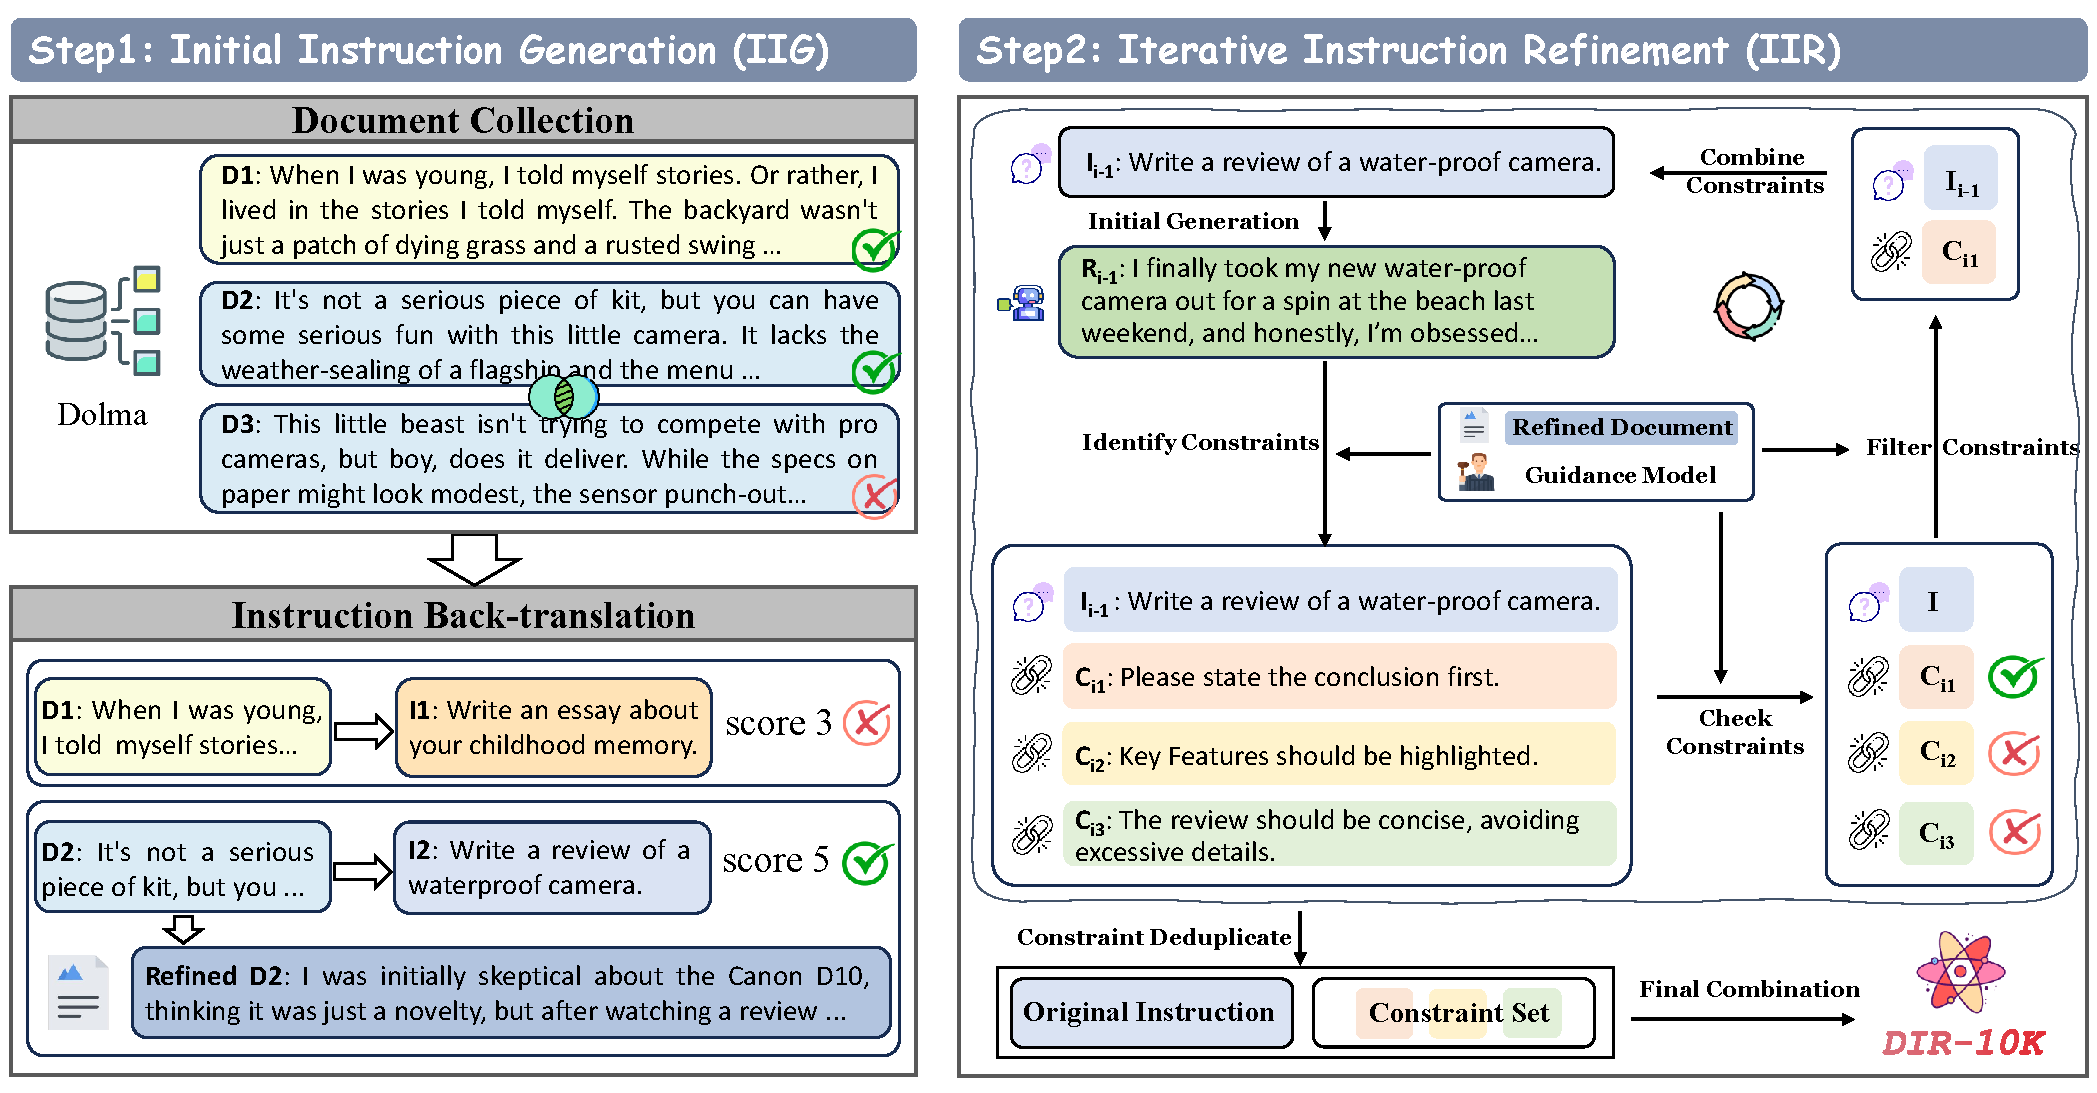
\includegraphics[width=1.0\linewidth]{source/main.pdf}
    \caption{
     DIR: Document-grounded Iterative Refinement. In the IIG phase, a large number of documents are collected for deduplication, followed by quality filtering based on scores assigned by the guidance model. Initial instructions are then generated using back-translation. In the IIR phase, refined documents and model responses from each iteration are used to generate constraints, ensuring compliance with the requirements stated in Section \ref{sec:IIR}. This iterative process continues until a final constraint set is produced, which is further combined with the original instruction to form the ultimate instruction.
    }
    \label{fig:main}
\end{figure*}

\subsection{Initial Instruction Generation (IIG)}

\subsubsection{Document Collection}
\label{sec:document_collection}
Traditional instruction generation methods such as Self-Instruct \citep{wang2022self} often suffer from limited diversity, as the generated instructions are generally re-combinations of the provided few-shot examples. Therefore, we propose a novel back-translation approach to construct initial instructions based on human-written documents.

To ensure the diversity of the generated instructions, we implement a density-based sampling mechanism for documents, as shown in Algorithm \ref{Alg:density}. Specifically, we convert documents into vector representations using Sentence-Transformers\footnote{\texttt{sentence-transformers/all-MiniLM-L6-v2}.}, and perform sampling to maximize the density of samples in the representation space. In this way, we effectively eliminate redundant documents. Furthermore, this approach ensures that the knowledge introduced in the instructions is evenly distributed across various domains, which prevents the model from overfitting to a specific domain and mitigates the risk of catastrophic forgetting of fundamental capabilities. 

Additionally, to further ensure the quality of the document collection, we filter out documents based on the following criteria: 1) Length: Remove documents with fewer than 50 words or exceeding 2,048 words; 2) Symbol ratio: Remove documents where the proportion of symbols exceeds that of textual content; and 3) Redundancy: Remove documents containing repetitive paragraphs or excessive symbol repetitions.


\begin{algorithm}[t]
  \renewcommand{\algorithmicrequire}{\textbf{Input:}}
  \renewcommand{\algorithmicensure}{\textbf{Output:}}
  \caption{Density-based Document Sampling}
  \begin{algorithmic}[1]
      \REQUIRE Initial collection $D$ with $m$ documents, number of documents to select $n$. 
      \ENSURE Selected collection $D'$ with $n$ documents.
      \STATE Derive the embeddings for each document in $D$.
      \STATE Randomly sample one document $x$ from $D$.
      \STATE Delete $x$ from $D$, add $x$ to $D'$.
      \FOR{$i = 1, 2, ..., n-1$}
          \STATE Calculate the cosine similarity score between $x$ and each document from $D$.
          \STATE Select the least similar document $x'$ from $D$.
          \STATE Let $x$ = $x'$.
          \STATE Delete $x$ from $D$, add $x$ to $D'$. 
      \ENDFOR
  \end{algorithmic}
\label{Alg:density}
\end{algorithm}

\subsubsection{Instruction Back-translation}
Based on the sampled documents, we employ a back-translation \citep{li2023self} method to construct initial instructions. Specifically, we utilize a proprietary guidance model\footnote{The guidance model is a proprietary LLM that is significantly stronger than the base model, as detailed in Section \ref{sec:models}.} to predict an instruction that can be answered with the document. This enables the generation of new instructions without relying on few-shot examples or pre-designed rules. Moreover, we can further ensure the diversity of the generated instructions by diversifying the documents.

Despite being derived from documents, the instructions do not always align well with the original document for two reasons. First, the documents are unstructured and do not conform to the AI-assistant format. Second, the documents may contain information irrelevant to the instruction ~\citep{nguyen2024better}. Therefore, we introduce a refinement step to transform the documents into response format and remove irrelevant content.

To further ensure data quality, we introduce a scoring step to filter out low-quality instructions. Each instruction is assigned a score on a scale of $1$ to $5$ by the guidance model, with each point corresponding to a specific dimension. Only instructions with a score of 4 or above are retained for the next step.

% \footnote{Instruction score criteria are presented in Appendix \ref{appendix:ins_score_case}.}

\subsection{Iterative Instruction Refinement (IIR)}
\label{sec:IIR}
To enhance a model’s ability to follow complex instructions, it is crucial to construct complex instruction data with multi-faceted constraints. Previous methods typically start with simple instructions and generate complex ones through rewriting~\citep{xu2023wizardlm}. However, the constraints generated in this way often do not meet actual needs or lack diversity.

% Therefore, we iteratively refine instructions by emulating the real-world process where people iteratively review responses and add constraints to address their deficiencies. This approach helps in developing more effective and challenging instructions.

% In practice, constructing complex instructions usually involves iteratively reviewing the response and adding constraints to address its deficiencies.

An effective sample for complex instruction alignment should adhere to two key principles:

\begin{enumerate}[itemsep=1mm, parsep=0pt]
    \item Whether the model’s response originally misaligns with the constraint before it is added;
    \item Whether the model’s response still misaligns with the constraint after it is added.
\end{enumerate}

These constraints highlight the model’s weaknesses in handling complex instructions and require further improvement. Conversely, if a constraint does not meet these principles, it indicates that the constraint falls within the model’s current capabilities and does not require additional learning.

Therefore, we introduce constraint generation using LLM-judge guidance \citep{zheng2023judging}, which mimics the human process of iteratively refining prompts to form complex instructions. During the iteration process, this method leverages the guidance model to judge the current response and identifies the constraints that the model fails to satisfy, thereby expanding simple instructions into complex ones, as shown in Algorithm \ref{alg:iir}.

% With the refined document as $R$, this method expands simple instructions $Q_o$ into complex ones through the following steps\footnote{Detailed prompt templates are presented in Appendix \ref{appendix:prompt_iir}.}:

\begin{figure*}[pos=tbp]
\centering
\includegraphics[width=0.96\linewidth]{source/iteration_constraint_distribution.png}
\caption{Constraint type distribution on DIR-10K among different iterations.}
\label{figure:constraint_dist}
\end{figure*}

\begin{algorithm}[t]
  \renewcommand{\algorithmicrequire}{\textbf{Input:}}
  \renewcommand{\algorithmicensure}{\textbf{Output:}}
  \caption{Iterative Instruction Refinement}
  \label{alg:iir}
  \begin{algorithmic}[1]
      \REQUIRE Guidance model $M$, current model $m$, refined document $D$, initial instruction $I_0$.
      \ENSURE Constraint Sets $C_n$ and $C_n'$.
      \FOR{$i = 1, 2, ..., n$}
          \STATE Use $m$ to generate a response $R_i$ for the previous instruction $I_{i-1}$.
          \STATE Leverage $M$ as the judge, compare $R_i$ with $D$ to identify a new constraint $c_i$.
          \STATE Add $c_i$ to $C_n$.
          \STATE Add $c_i$ to $I_{i-1}$ to form a new instruction $I_i$.
          \STATE Use $m$ to generate a response $R_{i}'$ for $I_i$.
          \STATE Leverage $M$ as the judge, check whether $R_i'$ satisfies constraint $c_i$. If not, add $c_i$ to $C_n'$. 
      \ENDFOR
  \end{algorithmic}
\end{algorithm}

% \begin{enumerate}[itemsep=1mm, parsep=0pt]
%     \item Leverage current model to generate a answer $A_i$ for the instruction $Q_i$.
%     \item Leveraging a guidance model as the judge, compare the refined document $R$ with the model's response to identify a new constraint $c_i$.
%     \item Add the constraints to the question $Q_{i-1}$ to construct a new question $Q_i$.
%     \item Answer $Q_i$ using the current model to derive answer $A_i$.
%     \item Determine whether the constraint $C_i$ is satisfied by $A_i$. If not, add the constraint to $C_n$.
%     \item Repeat the above three steps for multiple rounds to uncover increasingly complex constraints, thereby increasing the difficulty and depth of the instructions.
% \end{enumerate}

Throughout the iterative judgment process, as the number of constraints increases, the model's response also improves, making the identification of new constraints more challenging. Therefore, we utilize the refined document as the reference answer for judgment. Human-written documents inherently contain vast amounts of knowledge and formatting conventions that reflect human preferences. By grounding the constraint-generation process in documents, we achieve constraints that align more closely with human preferences.

Finally, the constraint set is merged into a new instruction. Note that two constraint sets are derived: the first set $C_n$ satisfies Principle 1, while the second set $C_n'$, which includes an additional checking step, satisfies both Principle 1 and 2.
% \footnote{An example of the IIR process is presented in Appendix \ref{appendix:pipeline_case}.}
% \textcolor{red}{Notice our approach incorporates several measures to ensure efficiency and scalability when handling large-scale documents and multiple iterations, while demonstrating robustness to variations in document quality, as detailed in Appendix \ref{appendix:efficiency_scalability} and \ref{appendix:document_quality}.}



\subsection{Data Statistics of DIR-10K}

\begin{figure}[pos=htbp]
\centering
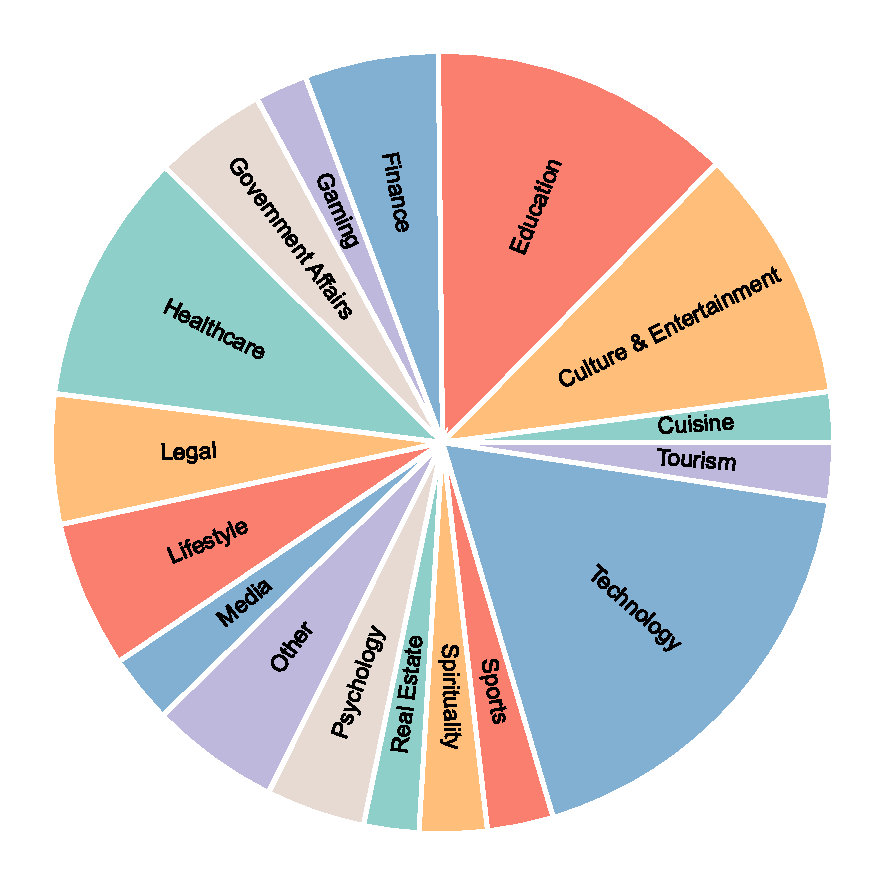
\includegraphics[width=0.6\linewidth]{source/data_visualization/domain_distribution.pdf}
\caption{Domain distribution on DIR-10K.}
\label{figure:domain_dist}
\end{figure}

\begin{figure}[pos=htbp]
\centering
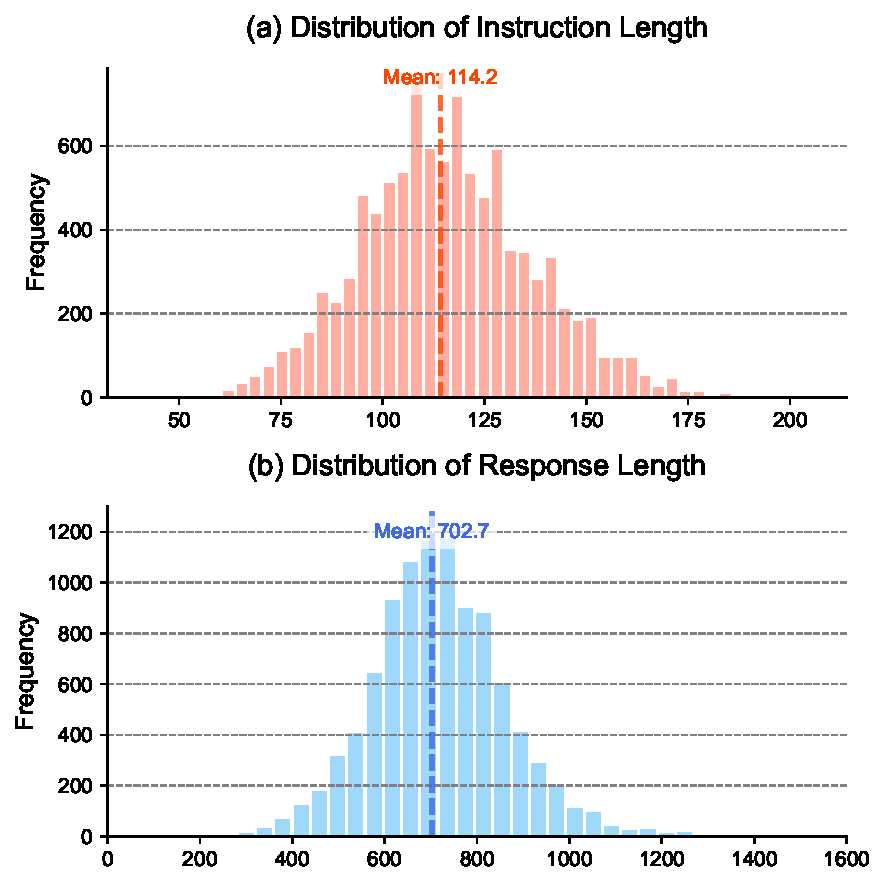
\includegraphics[width=0.78\linewidth]{source/data_visualization/length_distribution.pdf}
\caption{Distribution of instruction and response length on DIR-10K.}
\label{figure:length_dist}
\end{figure}

Utilizing our proposed framework, we constructed a high-quality complex instruction dataset, \textbf{DIR-10K}, based on openly available documents\footnote{We use a subset of Dolma v1.7 \citep{dolma-2024} following \citet{nguyen2024better}.}. Figure \ref{figure:constraint_dist} illustrates the evolution of constraint distributions across iterations (where a specific constraint type is specified for each generation). As can be seen, while \textit{Inclusion} and \textit{Document Structure} constraints predominate in the initial iteration, the distribution becomes progressively more uniform as iterations proceed. This validates that by uncovering constraints which are not covered by previous refinement iterations, our iterative refinement process effectively ensures constraint diversity.

We also present the domain distribution of DIR-10K in Figure \ref{figure:domain_dist}, following the domain definition in CFBench \citep{zhang2024cfbench}. As shown, our dataset encompasses nearly 20 different domains, exhibiting a high degree of balance across diverse fields. Furthermore, we analyzed the length distribution of the instructions using \textit{tiktoken}\footnote{We used \textit{o200k\_base} tokenizer for length calculation.}. As shown in Figure \ref{figure:length_dist}, the instruction lengths are primarily concentrated between 75 and 150 tokens, while the response lengths can scale to around 700 tokens, ensuring that our instructions provide sufficient information for aligning with complex instructions.